\documentclass[12pt,a4paper]{article}
\usepackage{styles/preamble}

% =================================================
% НАЧАЛО ДОКУМЕНТА
% =================================================

\begin{document}

\import{titlepage/}{title_old} % Титульный лист
\import{titlepage/}{title_new} % Титульный лист

\tableofcontents

\section{Самая главная секция}

На первых двух страницах приведены два варианта титульника: старый и новый. Далее приведён возможный вариант стил

\subsection{Шрифт}

В качестве шрифтов используются \href{https://fonts.google.com/specimen/Raleway}{Raleway} и \href{https://fonts.google.com/specimen/Anonymous+Pro}{AnonymousPro}.

\begin{itemize}
	\item Обычный начертаник, regular font.
	\item \textit{Курсивное начертание, italic font.}
	\item \textbf{Жирное начертание, bold font.}
	\item \texttt{Моноширное начертание, mono font.}
\end{itemize}

\subsection{Математические формулы}

В качестве примера приведена формула интегрирования по частям для определённого интеграла \eqref{simple_equation}.

\begin{equation} \label{simple_equation}
\int\limits_a^b u dv = uv \Big|_a^b - \int\limits_a^b v du
\end{equation} 

\subsection{Листинг}

В качестве примера приведена простая программа на языке Python (Листинг~\ref{listing:simple_code}).

\begin{minted}
[
	fontfamily=tt,
	numberblanklines=true,
	numbersep=5pt,
	frame=leftline,
	framerule=0.4pt,
	framesep=2mm,
	funcnamehighlighting=true,
	tabsize=4,
	breaklines=true,
	linenos=true,
	breakanywhere=true,
	bgcolor=LightGray,
]{python}
def main():
    greet('Sanya')

def greet(name):
    print('Hello, {}!'.format(name))

if __name__ == '__main__':
    main()
\end{minted}
\captionof{listing}{Простая программа на Python}
\label{listing:simple_code}

\newpage

\subsection{Картинка}

Можно вставлять картинки. Я так и сделал (Рис.~\ref{pic:luthadel}).
\begin{figure}[!h]
	\centering
	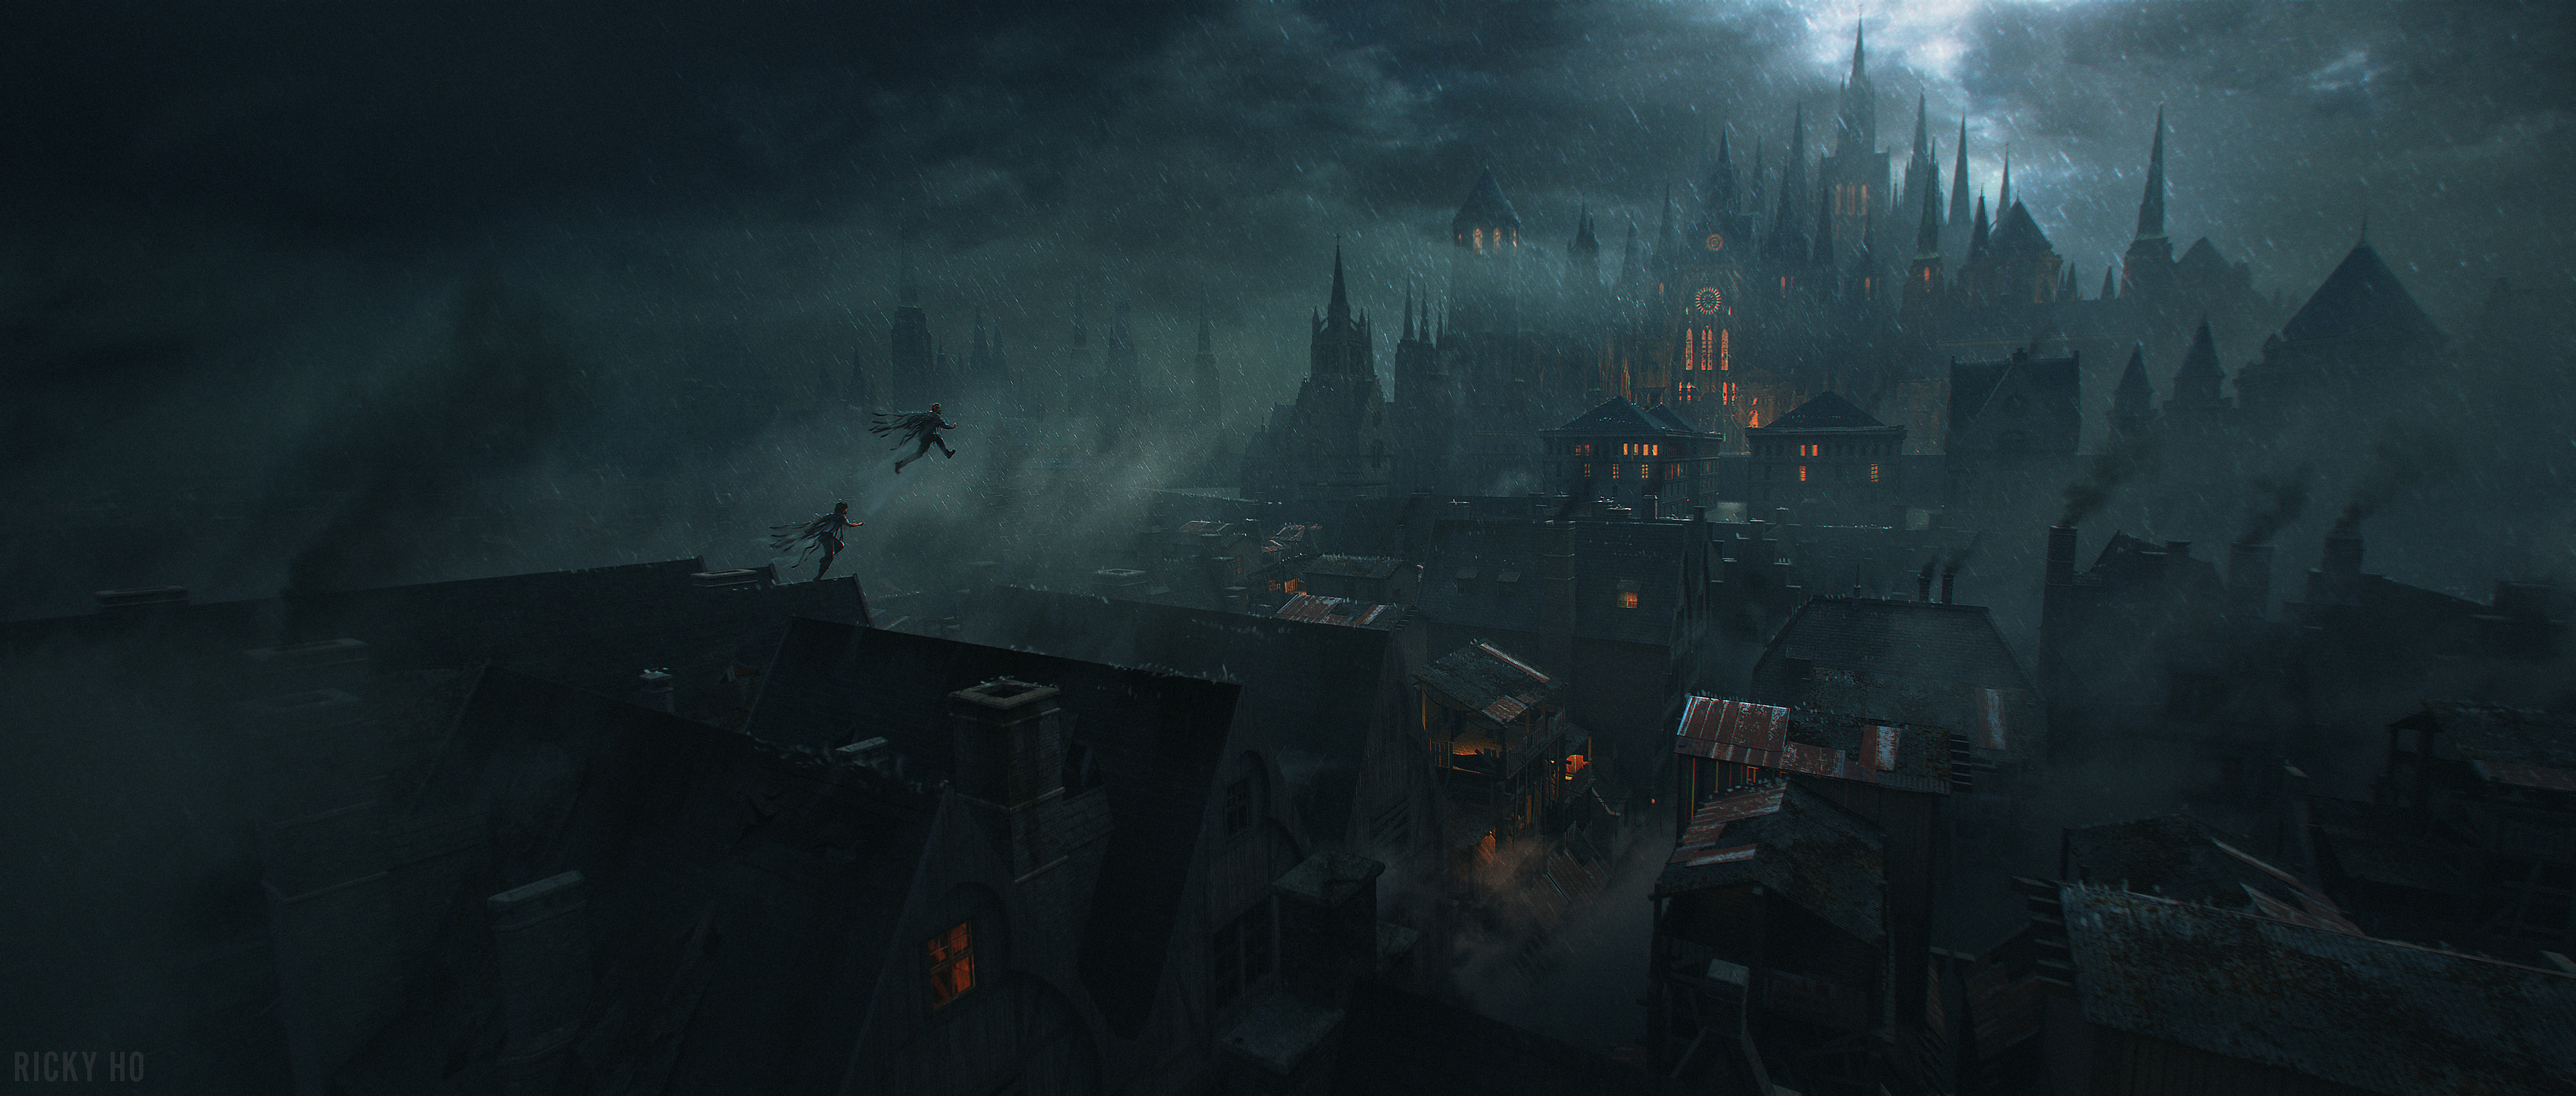
\includegraphics[width=1.0\textwidth]{pic/ricky-ho-mistborn-luthadel-city-rickyho}
	\caption{Mistborn: Luthadel at night by Ricky Ho}
	\label{pic:luthadel}
\end{figure}

\end{document}